% !TeX program = pdflatex
\documentclass[11pt,a4paper]{article}
\usepackage[utf8]{inputenc}
\usepackage[T1]{fontenc}
\usepackage[turkish]{babel}
\usepackage{lmodern}
\usepackage{geometry}
\usepackage{graphicx}
\usepackage{float}
\usepackage[section]{placeins}
\usepackage{flafter}
\usepackage{caption}
\usepackage{subcaption}
\usepackage{booktabs}
\usepackage{longtable}
\usepackage{hyperref}
\usepackage{xcolor}
\usepackage{microtype}
\usepackage{etoolbox}
\usepackage{amsmath,amssymb}
\usepackage{apacite}

\geometry{margin=1.8cm}
\graphicspath{{../results/}}
\setkeys{Gin}{width=0.95\linewidth, keepaspectratio}
\captionsetup{font=small,labelfont=bf}
\floatplacement{figure}{H}
\floatplacement{table}{H}
\preto\section{\FloatBarrier}
\preto\subsection{\FloatBarrier}
\AfterEndEnvironment{figure}{\FloatBarrier}
\AfterEndEnvironment{table}{\FloatBarrier}
\AfterEndEnvironment{longtable}{\FloatBarrier}

\title{Yazılım Tedarik Zincirinde Kritiklik Haritalaması:\\En Çok İndirilen 1000 NPM Paketinin Bağımlılıklarının Topolojik Risk Değerlendirmesi }
\author{\textbf{Yusuf Talha ARABACI}\\Karabük Üniversitesi\\Yüksek Lisans, Yazılım Mühendisliği Öğrencisi}
\date{Ekim 2025}

\begin{document}
\maketitle

\begin{abstract}
NPM ekosisteminde tek bir bağımlılıktaki kusur veya kötü niyetli değişiklik, transitif bağımlılıklar üzerinden geniş bir etki alanına yayılabilir. Bu bildiri, paket içeriklerinden ziyade paketler arası ilişkilerin \emph{topolojik} yapısına odaklanır. Bağımlı~$\to$~bağımlılık yönünde kurulan yönlü ağ üzerinde in-degree, out-degree ve betweenness merkeziyetleri hesaplanır; bu ölçüler min–max normalizasyonu ile bir \emph{bileşik risk skoru}na dönüştürülür. Ayrıca, en kritik düğümlerin çıkarılmasıyla ağın bağlanırlığı üzerinden bir \emph{sağlamlık} değerlendirmesi yapılır. Tüm görseller ve tablolar results/ dizinindeki çıktılara dayanır ve ilgili başlıklar altında sunulur.
\end{abstract}

\clearpage

\section{Giriş}
Yazılım tedarik zincirinde tek bir bağımlılıktaki hata ya da kasıtlı kötü niyetli değişiklik, transitif bağımlılıklar üzerinden yüzlerce hatta binlerce projeye yayılabilir. NPM ekosistemi; ölçek, sürüm sıklığı ve yoğun bağımlılık grafiği nedeniyle bu tür zincirleme risklere özellikle açıktır. Bu çalışma, paket içeriğinden ziyade paketler arası ilişkinin \emph{topolojik} yapısına odaklanır: Bir paketin ağ içindeki konumu ve bu konumun sistemik etkileri nicel olarak değerlendirilir. Amaç, topolojik ölçütleri tek bir bileşik skorda birleştirerek kritik paketleri önceliklendirmek ve ağ düzeyinde sağlamlık duyarlılıklarını görünür kılmaktır.\\Projenin kod ve özet sonuçları: \url{https://yusufarbc.github.io/npm-complex-network-analysis/}.

\section{Yöntem}
\subsection{Çalışma Tasarımı ve Parametreler}
Analiz, en çok indirilen ilk \textbf{1000} NPM paketinin oluşturduğu yönlü bağımlılık ağı üzerinde yürütülmüştür. Varsayılan ayarlar: betweenness için örnekleme (\(k\approx200\)), yalnızca \texttt{dependencies} alanı (isteğe bağlı \texttt{peerDependencies} dahil edilebilir), HTTP önbelleği ve tekrar denemeleri etkindir. Kenarlar \emph{bağımlı~$\to$~bağımlılık} yönündedir; graf yönlüdür (DiGraph).

\subsection{Veri Kaynakları ve Ön İşleme}
\begin{itemize}
  \item \textbf{Top N paket listesi:} Öncelik \texttt{ecosyste.ms} API’sinde (indirmeye göre), yedek olarak \texttt{npm registry search} ve \texttt{npms.io} kullanılır.
  \item \textbf{Paket adı kodlama:} Scoped paketler (\texttt{@scope/name}) için URL-güvenli kodlama uygulanır.
  \item \textbf{Sürüm seçimi:} \texttt{dist-tags.latest} mevcutsa o sürüm, değilse en yüksek sürüm anahtarı seçilir.
  \item \textbf{Önbellek ve tekrar:} Bağımlılık sorguları JSON dosyada önbelleklenir (\texttt{results/cache\_deps.json}); başarısız istekler en fazla üç kez tekrar edilir.
\end{itemize}

\subsection{Ağ Kurulumu}
\begin{itemize}
  \item Düğümler paketleri, kenarlar \emph{Dependent~$\to$~Dependency} yönünü temsil eder; self-loop yoktur, grafik yönlüdür.
  \item Paketlerin en güncel sürümlerinden \texttt{dependencies} alanı okunur; isteğe bağlı olarak \texttt{peerDependencies} dahil edilebilir.
  \item HTTP oturumu yeniden kullanılır; istekler basit tekrar (retry) ve disk önbelleği ile dayanıklı hale getirilir.
\end{itemize}

\subsection{Metrikler}
\begin{itemize}
  \item \textbf{in-degree}: Bir pakete bağımlı paket sayısı — çekirdek/merkez cazibeyi yansıtır.
  \item \textbf{out-degree}: Bir paketin bağlı olduğu bağımlılık sayısı — kırılgan yüzeyin genişliğini yansıtır.
  \item \textbf{betweenness centrality}: Akışın aralarından geçtiği köprü konumlar. Büyük graflarda örnekleme (\texttt{sample-k}) ile hızlandırılır.
\end{itemize}

\subsection{Normalizasyon ve Bileşik Risk}
Metrikler min–max ile [0,1] aralığına ölçeklenir: \(x' = (x-\min)/(\max-\min)\). Bileşik risk skoru:
\[
  \text{risk} = w_{in}\,in' + w_{out}\,out' + w_{btw}\,btw' \quad (\text{varsayılan: } 0.5,\,0.2,\,0.3)
\]
Ağırlıklar komut satırı seçenekleri ile değiştirilebilir. Betweenness büyük graflarda örnekleme (\(k\)) ile hesaplanır; tipik olarak \(k=200\) (graf boyutuna göre ayarlanır).

\subsection{Kaskad Etkisi (Basamaklanma) ve Sağlamlık}
\textbf{Kaskad etkisi.} Kenarlar \emph{Dependent~$\to$~Dependency} yönündeyken, bir bağımlılığın ele geçirilmesi onu \emph{kullanan} paketleri etkiler. Bu nedenle grafın tersinde (\(G^{\mathrm{rev}}\)) bir kaynaktan erişilebilen düğüm sayısı, o paketin potansiyel \emph{etki alanı}dır. Algoritma BFS/DFS ile \(O(|V|+|E|)\): \texttt{G\_rev = reverse(G); reach = BFS(G\_rev, s)}.

\textbf{Sağlamlık.} Seçili düğümler kaldırıldıktan sonra zayıf bağlı bileşen sayısı, en büyük bileşen boyutu ve (mümkünse) LCC çapı raporlanır. Bu ölçüler, kritik düğümlerin ağ bütünlüğüne etkisini gösterir.

\subsection{Köprü Kenarlar ve Diğer Çıktılar}
\textbf{Kenar betweenness.} Yüksek değere sahip kenarlar alt-ağlar arasında köprü görevi görür; kopmaları parçalanmayı hızlandırır. Ayrıca \texttt{edges.csv}, \texttt{metrics.csv}, \texttt{risk\_scores.csv} ve \texttt{graph\_stats.json} üretilir.

\section{Bulgular ve Yorum}
Bu bölümde bulgular görseller ve tablolarla birlikte, her birinin \emph{yorum} kısmıyla sunulmaktadır. Tüm materyal \texttt{results/} klasöründen alınmıştır.

\subsection{Ağ ve Derece Dağılımları}
\begin{figure}[H]
  \centering
  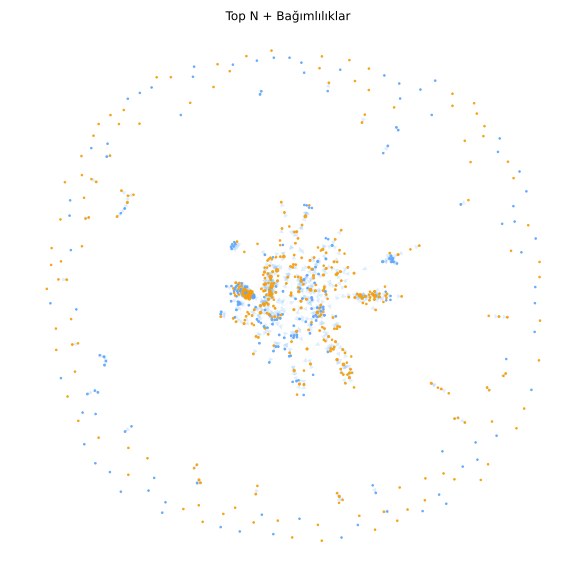
\includegraphics{network_full_topN.png}
  \caption{En çok indirilen paketlerle kurulan tam ağın görselleştirmesi. Yoğun merkezî bölgeler omurga paket kümelerini, seyrek bölgeler çevreyi işaret etmektedir.}
\end{figure}
\textit{Yorum —} Ağ görünümü, birkaç yüksek dereceli çekirdek etrafında yoğunlaşan küçük-dünya benzeri bir yapı sergiler. Bu, az sayıda paket üzerinde orantısız etki birikimine işaret eder.

\begin{figure}[H]
  \centering
  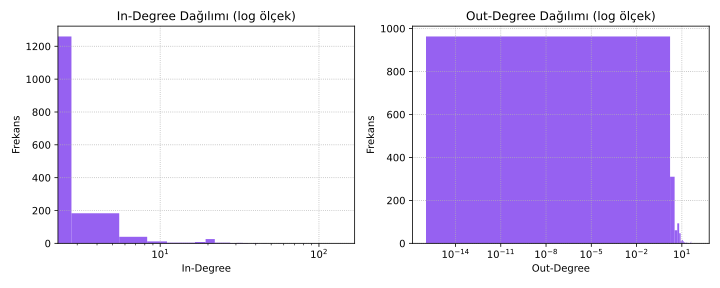
\includegraphics{degree_histograms.png}
  \caption{In-degree ve out-degree dağılımlarının histogramları. Her iki dağılım da ağır kuyruklu bir profil göstermektedir.}
\end{figure}
\textit{Yorum —} Ağır kuyruk, çok az sayıda paketin çok yüksek dereceye sahip olduğunu, büyük çoğunluğun ise düşük derecelerde kaldığını gösterir. Bu, sistemik riskte eşitsizliği artırır.

\subsection{Öncü Paketler ve Korelasyonlar}
\begin{figure}[H]
  \centering
  \includegraphics{top10_in_degree.png}
  \caption{In-degree açısından ilk 10 paket. Omurga niteliğindeki çekirdek bağımlılıklar.}
\end{figure}
\textit{Yorum —} Bu paketlerdeki bir bozulma, bağımlıların çokluğu nedeniyle zincirleme etkiler yaratabilir; bakım ve izleme önceliği yüksektir.

\begin{figure}[H]
  \centering
  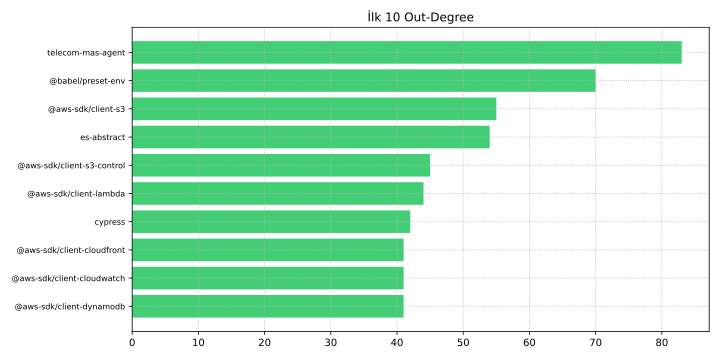
\includegraphics{top10_out_degree.png}
  \caption{Out-degree açısından ilk 10 paket. Geniş bağımlılık yüzeyine sahip bileşenler.}
\end{figure}
\textit{Yorum —} Yüksek out-degree, tedarik riskine duyarlılığı artırır; bu paketlerin alt bağımlılıklarında oluşan sorunlar doğrudan etkiler yaratır.

\begin{figure}[H]
  \centering
  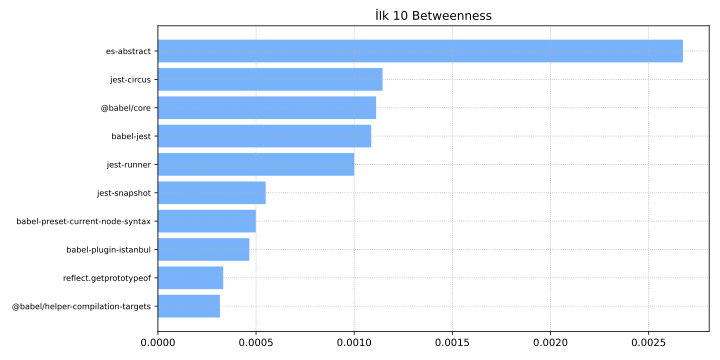
\includegraphics{top10_betweenness.png}
  \caption{Betweenness merkeziyeti açısından ilk 10 paket. Köprü/ana arter konumlar.}
\end{figure}
\textit{Yorum —} Köprü konumlar, alt-ağlar arasında akışın zorunlu geçtiği düğümler olup, hedefli saldırılara karşı hassastır.

\begin{figure}[H]
  \centering
  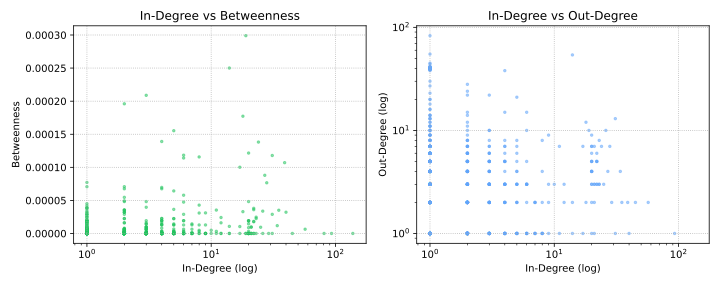
\includegraphics{scatter_correlations.png}
  \caption{Metrikler arası korelasyonlara ilişkin saçılım grafikleri. In-degree ile betweenness çoğu zaman birlikte yükselir; out-degree ilişkisi bağlama bağlıdır.}
\end{figure}
\textit{Yorum —} Korelasyonlar, tekil metriklerin farklı boyutları yakaladığını; bileşik skora ihtiyaç olduğunu doğrular.

\subsection{Bileşik Risk ve Kaskad Etki}
\begin{figure}[H]
  \centering
  \includegraphics{top20_risk.png}
  \caption{Bileşik risk skoruna göre ilk 20 paket. Ağırlıklar: in=0.5, out=0.2, btw=0.3.}
\end{figure}
\textit{Yorum —} Liste, yüksek in-degree ve betweenness kombinasyonuna sahip paketlerin üst sıraları domine ettiğini gösterir.

\begin{figure}[H]
  \centering
  \includegraphics{cascade_impact_top20.png}
  \caption{En riskli 20 paket için kaskad etki (ters yön dependents) büyüklükleri. Değerler, ters yön erişilebilir düğüm sayısını temsil eder.}
\end{figure}
\textit{Yorum —} Yüksek risk çoğunlukla daha geniş kaskadla örtüşse de, topolojiye bağlı istisnalar görülebilir.

\begin{figure}[H]
  \centering
  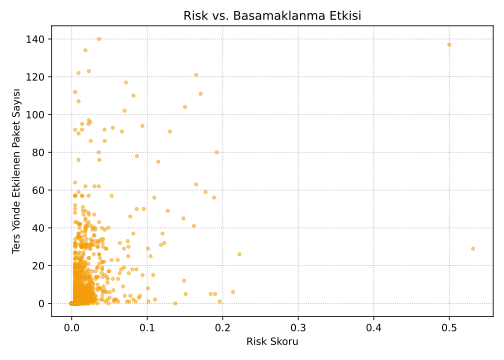
\includegraphics{risk_vs_cascade.png}
  \caption{Risk skoru ile kaskad etki (dependents yönü) ilişkisi. Doğrusal olmayan yapı, tek metrikle açıklamanın yetersizliğine işaret eder.}
\end{figure}
\textit{Yorum —} Kaskad etkisi, komşuluk yapısına duyarlıdır; benzer riskli düğümler farklı kaskad profilleri üretebilir.

\subsection{Tablolar: Derece ve Betweenness}
\noindent\textit{Yorum —} In-degree tablosu, omurga paketleri; out-degree tablosu, geniş bağımlılık yüzeyini; betweenness tablosu ise köprü konumları nicel olarak özetler.
\IfFileExists{../results/metrics_top20_in_degree.tex}{\begin{longtable}{lrrrr}
\caption{Top 20 In-Degree (Toplam Dugumler)}\\
\toprule
Paket & In-Degree & Out-Degree & Betweenness & TopN? \\
\midrule
\endfirsthead
\toprule
Paket & In-Degree & Out-Degree & Betweenness & TopN? \\
\midrule
\endhead
\bottomrule
\endfoot
\bottomrule
\endlastfoot
@babel/helper-plugin-utils & 110 & 0 & 0.000000 & True \\
call-bound & 41 & 2 & 0.000000 & False \\
postcss-value-parser & 39 & 0 & 0.000000 & True \\
call-bind & 36 & 4 & 0.000120 & False \\
@types/node & 34 & 1 & 0.000067 & False \\
debug & 34 & 1 & 0.000067 & True \\
es-errors & 33 & 0 & 0.000000 & False \\
@babel/types & 32 & 2 & 0.000175 & True \\
define-properties & 29 & 3 & 0.000067 & False \\
chalk & 28 & 0 & 0.000000 & False \\
@csstools/css-tokenizer & 27 & 0 & 0.000000 & False \\
@csstools/css-parser-algorithms & 26 & 0 & 0.000000 & False \\
@jest/types & 26 & 7 & 0.000211 & True \\
@csstools/utilities & 23 & 0 & 0.000000 & False \\
get-intrinsic & 22 & 10 & 0.000013 & True \\
jest-util & 22 & 6 & 0.000028 & True \\
graceful-fs & 21 & 0 & 0.000000 & False \\
postcss-selector-parser & 21 & 2 & 0.000000 & True \\
@babel/traverse & 20 & 7 & 0.000033 & True \\
es-object-atoms & 20 & 1 & 0.000000 & False \\
\end{longtable}
}{\fbox{metrics\_top20\_in\_degree.tex bulunamadı}}
\IfFileExists{../results/metrics_top20_out_degree.tex}{\begin{longtable}{lrrrr}
\caption{Top 20 Out-Degree (Toplam Dugumler)}\\
\toprule
Paket & Out-Degree & In-Degree & Betweenness & TopN? \\
\midrule
\endfirsthead
\toprule
Paket & Out-Degree & In-Degree & Betweenness & TopN? \\
\midrule
\endhead
\bottomrule
\endfoot
\bottomrule
\endlastfoot
telecom-mas-agent & 83 & 1 & 0.000000 & True \\
@babel/preset-env & 70 & 0 & 0.000000 & True \\
@aws-sdk/client-s3 & 55 & 1 & 0.000000 & False \\
es-abstract & 54 & 14 & 0.002503 & True \\
@aws-sdk/client-s3-control & 45 & 1 & 0.000000 & False \\
@aws-sdk/client-lambda & 44 & 1 & 0.000000 & False \\
cypress & 42 & 1 & 0.000000 & False \\
@aws-sdk/client-cloudfront & 41 & 1 & 0.000000 & False \\
@aws-sdk/client-cloudwatch & 41 & 1 & 0.000000 & False \\
@aws-sdk/client-dynamodb & 41 & 1 & 0.000000 & False \\
@aws-sdk/client-ec2 & 41 & 1 & 0.000000 & False \\
@aws-sdk/client-rds & 41 & 1 & 0.000000 & False \\
@aws-sdk/client-sqs & 41 & 1 & 0.000000 & False \\
@aws-sdk/client-cloudformation & 40 & 1 & 0.000000 & False \\
@aws-sdk/client-iam & 40 & 1 & 0.000000 & False \\
@aws-sdk/client-ses & 40 & 1 & 0.000000 & False \\
@aws-sdk/client-cloudhsm & 39 & 1 & 0.000000 & False \\
@aws-sdk/client-cloudsearch & 39 & 1 & 0.000000 & False \\
@aws-sdk/client-cloudtrail & 39 & 1 & 0.000000 & False \\
@aws-sdk/client-kms & 39 & 1 & 0.000000 & False \\
\end{longtable}
}{\fbox{metrics\_top20\_out\_degree.tex bulunamadı}}
\IfFileExists{../results/metrics_top20_betweenness.tex}{\begin{longtable}{lrrrr}
\caption{Top 20 Betweenness (Toplam Dugumler)}\\
\toprule
Paket & Betweenness & In-Degree & Out-Degree & TopN? \\
\midrule
\endfirsthead
\toprule
Paket & Betweenness & In-Degree & Out-Degree & TopN? \\
\midrule
\endhead
\bottomrule
\endfoot
\bottomrule
\endlastfoot
jest-snapshot & 0.000689 & 5 & 21 & True \\
jest & 0.000601 & 1 & 4 & True \\
@jest/core & 0.000481 & 2 & 28 & True \\
@jest/transform & 0.000322 & 6 & 15 & True \\
get-intrinsic & 0.000299 & 19 & 10 & True \\
cypress & 0.000259 & 1 & 42 & False \\
@babel/core & 0.000204 & 4 & 15 & True \\
side-channel & 0.000204 & 3 & 5 & True \\
@cypress/request & 0.000186 & 1 & 18 & False \\
jest-haste-map & 0.000182 & 6 & 10 & True \\
qs & 0.000176 & 8 & 1 & True \\
execa & 0.000174 & 2 & 12 & True \\
puppeteer & 0.000166 & 1 & 6 & False \\
@babel/helper-compilation-targets & 0.000161 & 6 & 5 & True \\
@babel/traverse & 0.000157 & 17 & 7 & True \\
@jest/types & 0.000157 & 24 & 7 & True \\
babel-preset-current-node-syntax & 0.000145 & 2 & 15 & True \\
babel-plugin-istanbul & 0.000142 & 2 & 5 & True \\
@babel/helper-create-class-features-plugin & 0.000141 & 5 & 7 & True \\
http-signature & 0.000141 & 2 & 3 & False \\
\end{longtable}
}{\fbox{metrics\_top20\_betweenness.tex bulunamadı}}

\subsection{Tablolar: Risk ve Kaskad}
\noindent\textit{Yorum —} Risk sıralaması, çok boyutlu kritiklik sinyalini tek bir ölçekte verir; kaskad tablosu, etki alanının büyüklüğünü gösterir.
\IfFileExists{../results/risk_scores_top20.tex}{\begin{longtable}{lrrrrr}
\caption{Top 20 Risk Skoru}\\
\toprule
Paket & Risk & In-Degree & Out-Degree & Betweenness & TopN? \\
\midrule
\endfirsthead
\toprule
Paket & Risk & In-Degree & Out-Degree & Betweenness & TopN? \\
\midrule
\endhead
\bottomrule
\endfoot
\bottomrule
\endlastfoot
tslib & 0.500000 & 138 & 0 & 0.000000 & True \\
es-abstract & 0.431785 & 14 & 54 & 0.000250 & True \\
get-intrinsic & 0.392937 & 19 & 10 & 0.000299 & True \\
@smithy/types & 0.339366 & 93 & 1 & 0.000000 & True \\
@babel/helper-plugin-utils & 0.293478 & 81 & 0 & 0.000000 & True \\
@aws-sdk/credential-provider-node & 0.271994 & 18 & 12 & 0.000177 & True \\
@aws-sdk/core & 0.261914 & 31 & 13 & 0.000118 & True \\
call-bound & 0.253485 & 39 & 2 & 0.000107 & True \\
@aws-sdk/nested-clients & 0.245554 & 4 & 38 & 0.000139 & False \\
@jest/types & 0.242459 & 24 & 7 & 0.000138 & True \\
side-channel & 0.232483 & 3 & 5 & 0.000209 & True \\
jest-snapshot & 0.224549 & 5 & 21 & 0.000155 & True \\
@puppeteer/browsers & 0.220782 & 2 & 7 & 0.000196 & False \\
@aws-sdk/types & 0.217789 & 57 & 2 & 0.000006 & True \\
jest-util & 0.208899 & 20 & 6 & 0.000122 & True \\
telecom-mas-agent & 0.203623 & 1 & 83 & 0.000000 & True \\
call-bind & 0.195697 & 27 & 4 & 0.000088 & True \\
@smithy/smithy-client & 0.195157 & 28 & 7 & 0.000077 & True \\
debug & 0.179578 & 40 & 1 & 0.000032 & True \\
@babel/traverse & 0.178945 & 17 & 7 & 0.000100 & True \\
\end{longtable}
}{\fbox{risk\_scores\_top20.tex bulunamadı}}
\IfFileExists{../results/cascade_impact_top20.tex}{\input{../results/cascade_impact_top20.tex}}{\fbox{cascade\_impact\_top20.tex bulunamadı}}

\subsection{Tablolar: Köprü Kenarlar}
\noindent\textit{Yorum —} Kenar betweenness sıralaması, parçalanmaya duyarlı bağlantıların tespitinde yol göstericidir.
\IfFileExists{../results/edge_betweenness_top10.tex}{\begin{longtable}{l l r}
\caption{Edge Betweenness Ilk 10 (Yuksek kopru kenarlar)}\\
\toprule
U & V & Edge Betweenness \\
\midrule
\endfirsthead
\toprule
U & V & Edge Betweenness \\
\midrule
\endhead
\bottomrule
\endfoot
\bottomrule
\endlastfoot
jest & @jest/core & 0.000142 \\
@jest/expect & jest-snapshot & 0.000100 \\
reflect.getprototypeof & which-builtin-type & 0.000094 \\
@jest/transform & babel-plugin-istanbul & 0.000086 \\
@babel/traverse & @babel/generator & 0.000082 \\
jest-snapshot & @jest/transform & 0.000081 \\
call-bound & get-intrinsic & 0.000081 \\
@babel/core & @babel/helper-compilation-targets & 0.000078 \\
telecom-mas-agent & jest & 0.000077 \\
jest-snapshot & babel-preset-current-node-syntax & 0.000076 \\
\end{longtable}
}{\fbox{edge\_betweenness\_top10.tex bulunamadı}}

\section{İlgili Çalışmalar ve Konumlandırma}
Tedarik zinciri tehdit taksonomileri, kötüye kullanım teknik haritaları ve bağımlılık ağlarının yapısal özelliklerini inceleyen zengin bir literatür bulunmaktadır. Örneğin \emph{Backstabbers Knife Collection} saldırı taksonomisi \cite{backstabbers2019}, \emph{Hitchhiker’s Guide} ekosistemler arası kurulum/çalışma zamanı tekniklerini \cite{hitchhikers2020}, \emph{OSCAR} gibi dinamik analiz hattı çalışmaları ise zehirleme tespitinde pratik iyileştirmeleri rapor eder \cite{oscar2023}. NPM bağımlılık ağlarının küçük-dünya özellikleri ve hedefli düğüm çıkarımlarındaki kırılganlık da daha önce sayısallaştırılmıştır \cite{npm_robustness,web_of_dependencies,demystifying}. Bu çalışma, söz konusu bulguları operasyonel bir \emph{yapısal risk} metriğinde birleştirip önceliklendirmeye odaklanmaktadır \cite{practical_malicious,supply_chain_attacks}.

\section{Tartışma ve Sınırlılıklar}
Betweenness merkeziyeti büyük graflarda hesaplama açısından pahalıdır; bu nedenle örnekleme kullanımı pratikte gereklidir. HTTP API yanıtlarındaki geçici hatalar eksik veri doğurabilir; önbellekleme ve tekrar denemeleri bu etkiyi azaltır. Risk ağırlıkları alan-bağımlıdır; bağlamınıza göre \(w_{in}, w_{out}, w_{btw}\) değerlerini yeniden kalibre etmeniz önerilir.

\section{Sonuç}
Bağımlılık topolojisinin merkeziliği ve köprü konumları, paket içi zafiyet göstergelerinin ötesinde yapısal bir risk perspektifi sunar. Burada sunulan basit ama yorumlanabilir bileşik skor, sınırlı analiz kapasitesini yüksek etkili paketlere yönlendirmek için kullanılabilir. Gelecek çalışmalar, sayfa-derecesi (PageRank), k-çekirdek ya da topluluk/çekirdek ayrışımı gibi ek metriklerle skoru zenginleştirebilir.

\section*{Çıktılar ve Tekrarlanabilirlik}
Tam çıktı listesi ve görseller için \texttt{results/} klasörüne bakınız. CLI tekrarı:
\begin{quote}
\texttt{python -m analysis.run --topN 1000 --sample-k 200 --classify}
\end{quote}

\bibliographystyle{apacite}
\bibliography{references}

\end{document}

